\documentclass[twocolumn]{article}
\usepackage[utf8]{inputenc}
\usepackage[margin=1in]{geometry}  % 调整页面边距
\usepackage{titling}               % 控制标题位置
\usepackage{booktabs}              % 表格宏包
\usepackage{amssymb}
% \usepackage{ctex}                  % 中文支持包
\usepackage{authblk}			   % 多作者
\usepackage{graphicx}
\usepackage{ragged2e}           % 摘要两端对齐
% \usepackage{tabularx}			% 表格宽度
% \usepackage{xeCJK}
\setlength{\droptitle}{-3.0cm}     % 将标题上移3.0厘米

\title{A Multi-stage Cascaded Encoder-decoder Framework for CT-to-PET Image Conversion in Lung Imaging}
\author[1] {Xiaoyu Deng}
\author[1,2] {Kouki Nagamune}
\author[1] {Hiroki Takada}
% \author[1] {Teacher Author}
% \author[1,3]{Third Author}
\affil[1]{University of Fukui, 3-9-1 Bunkyo, Fukui, 910-0019, Japan}
\affil[2]{University of Hyogo, 2167 Shosha, Himeji, Hyogo, 670-2280, Japan}
% \affil[3]{Research Institute, Company Z}
\date{ }

\begin{document}

\twocolumn[
	\maketitle

	\begin{center}
		\begin{abstract}
			\begin{justify}
				U-Net, a widely recognized deep learning architecture, excels in medical image processing tasks due to its symmetric encoder-decoder structure and skip connections, effectively preserving spatial information critical for precise segmentation. Although enlarging U-Net through depth increments, additional channels, improved skip connections, or integrating attention mechanisms such as Transformers can boost performance, it also introduces computational complexity and performance bottlenecks.

				This study proposes a multi-stage cascaded framework utilizing sequentially connected simple encoder-decoder modules for the CT-to-PET medical image translation task, preserving simplicity within each encoder-decoder structure. The effectiveness of the framework is validated experimentally using publicly available lung cancer PET-CT datasets, assessing performance across various stages. Metrics including SSIM, PSNR, and MAE demonstrate significant improvements in image reconstruction quality, particularly at higher cascade stages, achieving peak SSIM of 0.9255 and PSNR of 28.9168 dB.

				Visual comparison further indicates that despite high quantitative metric scores, certain visual artifacts remain due to transposed convolution operations, suggesting that pixel-level metrics alone may not comprehensively reflect perceptual quality. The proposed multi-stage cascaded U-Net model, therefore, presents strong potential for medical imaging applications, particularly in synthesizing high-quality PET images from CT scans, with recommendations for future integration of visual quality assessments and expert evaluations.
			\end{justify}
		\end{abstract}
	\end{center}
	\vspace{0.5cm}  % 调整摘要与正文之间的间距
]

\section{Introduce}
U-Net is a deep learning architecture originally designed for segmentation tasks. Due to its outstanding performance and efficient structure, it has become highly popular in medical image processing. U-Net improves upon traditional convolutional neural networks (CNNs) through a symmetric "U"-shaped architecture, consisting of a contracting path (encoder) and an expansive path (decoder), also known as an encoder-decoder structure. A crucial feature of U-Net is its use of skip connections, which connect feature maps from the contracting path to corresponding layers in the expansive path. This design enables the network to leverage precise spatial information during upsampling, significantly enhancing the accuracy of segmentation boundaries, particularly important in medical imaging where structural delineation is critical.

Increasing the scale of U-Net models can involve deepening the network, increasing the number of feature map channels, improving skip connection structures, and incorporating attention modules like Transformers. While these enhancements can improve performance, they also increase model complexity and computational demands, often leading to performance bottlenecks. In this research, multiple simple encoder-decoder structures are used to construct a generative network, verifying the performance of multi-stage models in medical image generation tasks.

The main contributions of this paper include proposing a multi-stage cascaded extension framework, constructing multiple multi-stage cascade models with simple encoder-decoder modules for CT-to-PET image conversion tasks, validating the effectiveness of this framework through experiments, and presenting performance metrics across various stages. The specific contributions are:

Proposing a multi-stage cascaded framework utilizing multiple simple encoder-decoder models for lung CT-to-PET image conversion tasks without altering individual encoder-decoder structures.

Experimentally validating the effectiveness of the proposed framework on publicly available paired PET-CT datasets, showcasing the performance of U-Net models at each stage, and monitoring various training and testing metrics.

Visually comparing images generated by different cascade models against real images to explore the effect of cascading on visual quality.

\section{Related Works}
Since the introduction of U-Net by Olaf et al. \cite{navab_u-net_2015}, it has been extensively employed due to its structural advantages and excellent performance in applications such as image denoising, medical image registration, and attenuation correction. It has also been applied in various other segmentation tasks including lesion segmentation and facial image restoration.

Armanious et al. \cite{armanious_medgan_2020} proposed an end-to-end GAN-based framework for medical image-to-image translation, demonstrating its performance in PET-CT translation, MR motion artifact correction, and PET denoising tasks. Singh et al. \cite{singh_automated_2023} presented a U-Net-based automated medical image registration method, employing GAN to generate pseudo-CT images from non-attenuation-corrected PET images, enhancing coronary angiography registration accuracy. Liu et al. \cite{liu_deep_2018} developed a method for generating pseudo-CT images for attenuation correction from single non-attenuation-corrected 18F-FDG PET images. Du et al. \cite{du_medical_2020} reviewed six U-Net-based methods for medical image segmentation, including lung nodules, cardiac, and brain segmentation tasks. Zeng et al. \cite{zeng_swin-casunet_2022} used a two-stage cascaded U-Net for facial image restoration, indicating potential advantages of multi-stage U-Net models for image generation tasks. Singh and Liu applied models with fine-tuned modules in medical image registration and attenuation correction, achieving notable results. While Armanious and Zeng utilized cascaded U-Net structures, multi-stage cascaded U-Net models for medical image generation remain underexplored. This study evaluates multi-stage cascaded U-Net models for CT-to-PET image conversion tasks using several metrics.

The Structural Similarity Index (SSIM) measures structural similarity between two images, considering luminance, contrast, and structural information, ranging from -1 to 1, with 1 indicating identical images. The Multi-scale SSIM (MS-SSIM) extends SSIM across multiple scales, better assessing image quality across varying resolutions. Peak Signal-to-Noise Ratio (PSNR) measures image reconstruction quality by comparing original and processed images, widely used in signal processing applications. Mean Absolute Error (MAE) computes the average pixel intensity difference between reconstructed and original images, insensitive to outliers compared to Mean Squared Error (MSE), thus selected as an evaluation metric given pixel scaling between 0 and 1 in PyTorch frameworks.


\section{Method}
The encoder-decoder architecture symmetrically captures context via a contracting path and achieves precise localization via an expansive path. This study constructs a standard U-Net convolutional neural network to convert CT images to PET images, optimized using a task-specific loss function.

The proposed cascaded framework comprises encoder, decoder, and visualization modules. The encoder extracts image features, the decoder reconstructs these features into output images, and the visualization module converts outputs into analyzable visual results. The detailed encoder-decoder structure is shown in Figure \ref{fig:Encoder_Decoder_Pair}.

% % TODO: \usepackage{graphicx} required
\begin{figure*}[t!]
	\centering
	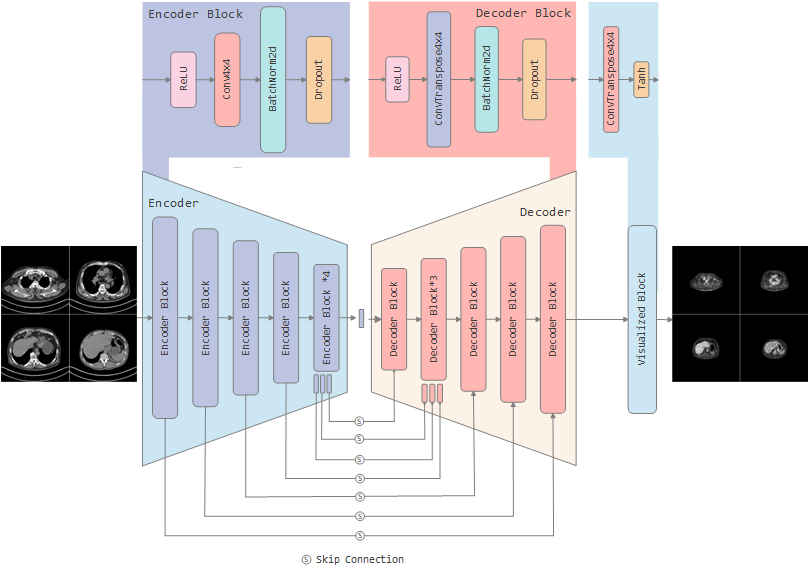
\includegraphics[width=1.0\linewidth]{u-net/lung/Encoder-Decoder-5layer-250406}
	\caption[architecture]{Schematic Diagram of Data Flow Within the Model. The PET image is shown on the left, and the CT image on the right. The blue modules correspond to the encoder architecture, while the orange modules represent the decoder architecture. The upper portion of the figure illustrates the fundamental structures of the encoder blocks, decoder blocks, and visualization blocks. The connections in the lower portion indicate the skip connections.}
	\label{fig:Encoder_Decoder_Pair}
\end{figure*}

\textbf{Encoder Block} The encoder follows the typical architecture of a convolutional network. It consists of repeated application of two $3\times3$ convolutions, each followed by a rectified linear unit (ReLU) and a $2\times2$ max pooling operation with stride 2 for downsampling. At each downsampling step, the number of feature channels is doubled. The convolution operation in U-Net can be described by the following equation:
\[
	I' = \sum_{i,j} (I * K)(i,j) + b
\]
where \(I\) represents the input image, \(K\) is the convolution kernel, \(b\) is the bias, and \(I'\) is the output feature map.

\textbf{Decoder Block} The decoder includes a series of upsampling and convolution operations. Each step in the expanding path includes an upsampling of the feature map followed by a $2\times2$ convolution that halves the number of feature channels, a concatenation with the correspondingly cropped feature map from the contracting path, and two $3\times3$ convolutions, each followed by a ReLU. Up sampling in the expanding path uses transposed convolutions to increase the size of the feature map:
\[
	U = K^T * I
\]
where \(K^T\) is the transposed convolution kernel and \(U\) is the upsampled output.

\textbf{Visual Block} module, a variant decoder, converts output features from the decoder module into a visual format. Its structure is similar to a standard decoder but lacks skip connections and employs different nonlinear functions, enhancing visual analysis.

\begin{table}[h]
	% \centering
	\caption{Encoder-decoder Setting Table}
	\label{tab:encoder_setting}
	\begin{tabular}{ccccc}
		\hline
		Block Name   & input & output & trans & dropout \\
		\hline
		Encoder 1    & 3     & 64     & -     & -       \\
		Encoder 2    & 64    & 128    & -     & -       \\
		Encoder 3    & 128   & 512    & -     & -       \\
		Encoder 4    & 256   & 512    & -     & -       \\
		Encoder 5    & 512   & 512    & -     & -       \\
		Encoder 6    & 512   & 512    & -     & -       \\
		Encoder 7    & 512   & 512    & -     & -       \\
		Encoder 8    & 512   & 512    & -     & -       \\
		Decoder 1    & 512   & 1024   & 512   & 0.5     \\
		Decoder 2    & 1024  & 1024   & 512   & 0.5     \\
		Decoder 3    & 1024  & 1024   & 512   & 0.5     \\
		Decoder 4    & 1024  & 1024   & 512   & -       \\
		Decoder 5    & 1024  & 512    & 256   & -       \\
		Decoder 6    & 512   & 256    & 128   & -       \\
		Decoder 7    & 256   & 128    & 64    & -       \\
		Visual Block & 128   & 3      & -     & -       \\
		\hline
	\end{tabular}
\end{table}


\begin{table}[h]
	\centering
	\caption{Parameters of Neural Networks.}
	\label{tab:model_parameters}
	\begin{tabular}{ccccc}
		\hline
		Architectures & Parameters \\
		\hline
		% Stage01       & 54.41      \\
		% Stage02       & 108.82     \\
		% DualSG      & 92.54      \\
		Stage03       & 163.24     \\
		Stage04       & 217.66     \\
		Stage05       & 272.07     \\
		Stage06       & 326.49     \\
		Stage07       & 380.90     \\
		Stage08       & 435.31     \\
		Stage09       & 489.73     \\
		Stage10       & 544.155    \\
		\hline
		\multicolumn{2}{p{201pt}}{The table depicts the Parameters of different generators. The quantity of parameters is expressed in millions.}
	\end{tabular}
\end{table}

\subsection{Cascaded Expansion Framework}

This study introduces a cascaded expansion framework using multiple encoder-decoder structures cascaded sequentially. Each encoder-decoder output becomes the input for the subsequent stage, refining features progressively. This approach enhances model accuracy by capturing richer feature information at each stage. Although theoretically possible, segmented optimization strategies for different stages are not explored further here. Additionally, a Dual Stage Generator GAN (DSGGAN) with dense connections and segmented optimization mechanisms is introduced to capture stage-specific features more effectively. Table \ref{tab:model_parameters} details model parameter counts.




\section{Experiments}
This study employs the encoder-decoer architecture for cross-modality medical image conversion tasks, specifically to construct a U-Net that inputs a CT image and converts it into a corresponding PET image. In this research, the lung PET or CT scan data were powered by the National Cancer Institute Cancer Imaging Program (CIP) \cite{li_large-scale_2020}.  The dataset encompasses 251,135 lung scan images from 355 subjects, primarily collected between 2009 and 2011, including each subject's gender, age, weight, smoking history, and cancer diagnosis classification. All scan data in the dataset are stored in DICOM format. This study processed these 251,135 scan data using the MicroDicom software on a Windows operating system. The subjects in the dataset are labeled according to the type of cancer: Type A for adenocarcinoma, Type B for small cell carcinoma, Type E for large cell carcinoma, and Type G for squamous cell carcinoma. Not all subjects' data include both PET and CT scans. Therefore, this study selected imaging data from 38 confirmed Type B small cell carcinoma patients, including PET scans with CT scans, and fused enhanced images, resulting in 464 PET/CT pairs. Data was divided into trainingand testing sets, detailed in Table \ref{tab:dataset_partition_1}.

% 插入三线表
\begin{table}[h]
	\centering
	\caption{Dataset Partition of Experiment}
	\label{tab:dataset_partition_1}
	\begin{tabular}{cccc}
		\toprule
		Params count     & Test & Train & Total \\
		\midrule
		Lung PET/CT Pair & 64   & 400   & 464   \\
		Total Images     & 128  & 800   & 928   \\
		\bottomrule
	\end{tabular}
\end{table}

The optimization employed Mean Squared Error and adversarial loss functions, utilizing Adam optimizer with a learning rate of 0.001 for gradual convergence. Optimal experimental results are listed in Table \ref{tab:exps_result}.

\begin{table}[h]
	\centering
	\caption{Max SSIM,PSNR,MAE Results of Experiment}
	\label{tab:exps_result}
	\begin{tabular}{cccc}
		\toprule
		Stage Count & SSIM            & PSNR             & MAE             \\
		\midrule
		U-Net       & 0.9149          & 27.7411          & 0.0119          \\
		Cas-Unet    & 0.9182          & 27.9950          & 0.0109          \\
		DSGGAN      & 0.9122          & 28.7630          & 0.0105          \\
		3 Stages    & 0.9060          & 27.6395          & 0.0127          \\
		4 Stages    & 0.9155          & 28.1969          & 0.0112          \\
		5 Stages    & 0.9104          & 26.6691          & 0.0130          \\
		6 Stages    & 0.9167          & 27.9794          & 0.0108          \\
		7 Stages    & \textbf{0.9255} & 27.1919          & 0.0116          \\
		8 Stages    & 0.9178          & 28.5503          & 0.0107          \\
		9 Stages    & 0.9093          & 28.7770          & 0.0109          \\
		10 Stages   & 0.9245          & \textbf{28.9168} & \textbf{0.0097} \\

		\bottomrule
	\end{tabular}
\end{table}

Metrics including SSIM, PSNR, and MSE were recorded over 200 training epochs, revealing high performance across training and testing datasets. Stage07 and Stage10 models exhibited higher SSIM and PSNR values, indicating superior reconstruction quality.

\begin{figure}[h]
	\centering
	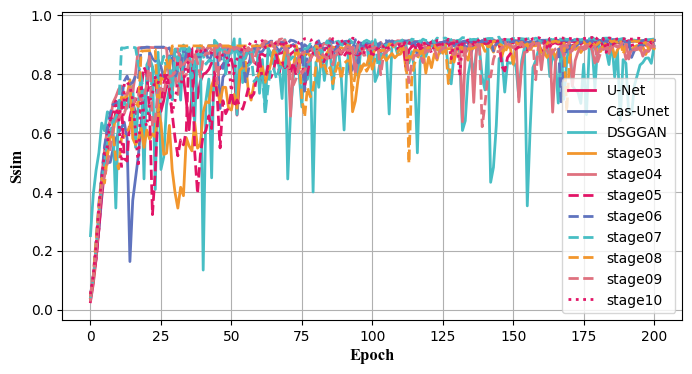
\includegraphics[width=1.0\linewidth]{u-net/lung/csv_lung_13_csv_img_2025_04_07_01_44_03/ssim_comparison}
	\caption[ssim]{SSIM Line Figure of All Epoch in Test Process}
	\label{fig:ssim}
\end{figure}

Figure \ref{fig:ssim} illustrates SSIM rapidly increasing in initial training (first 25 epochs), stabilizing around 0.9. DSGGAN exhibited fluctuations possibly due to overemphasis on high-dimensional features, but overall SSIM remained high.

\begin{figure}[h]
	\centering
	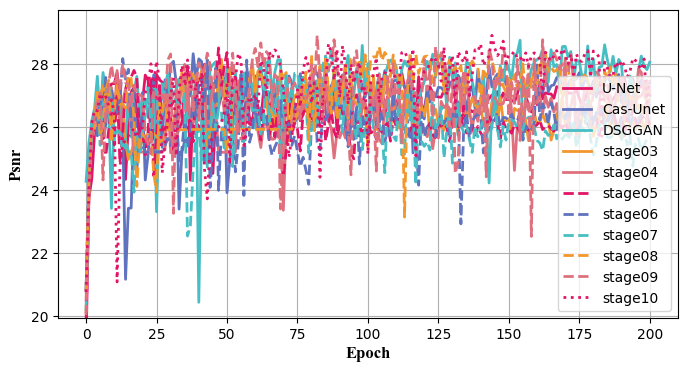
\includegraphics[width=1.0\linewidth]{u-net/lung/csv_lung_13_csv_img_2025_04_07_01_44_03/psnr_comparison}
	\caption[psnr]{PSNR Line Figure of All Epoch in Test Process}
	\label{fig:psnr}
\end{figure}

PSNR (Figure \ref{fig:psnr}) showed rapid initial improvements with subsequent fluctuations, particularly in 8-, 6-, and 5-stage models, indicating potential generalization issues with complex data or smaller datasets. Overall, PSNR remained consistently good.

\begin{figure}[h]
	\centering
	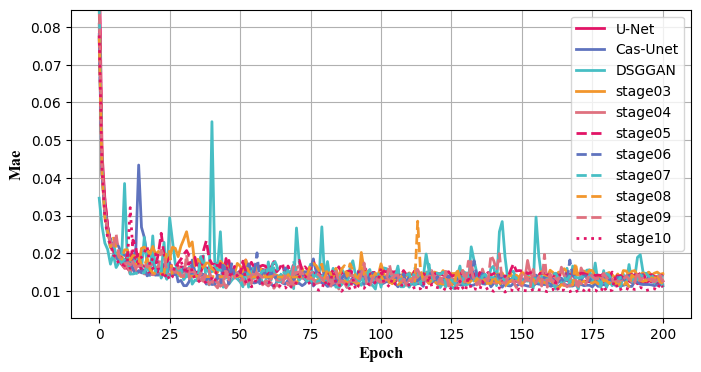
\includegraphics[width=1.0\linewidth]{u-net/lung/csv_lung_13_csv_img_2025_04_07_01_44_03/mae_comparison}
	\caption[mae]{MAE Line Figure of All Epoch in Train and Test Process}
	\label{fig:mae}
\end{figure}

MAE (Figure \ref{fig:mae}) initially dropped rapidly, demonstrating effective adaptation. Occasional spikes in DSGGAN and 3-stage models occurred possibly due to distinct skip connection designs, yet overall remained low.


\begin{figure*}[h]
	\centering
	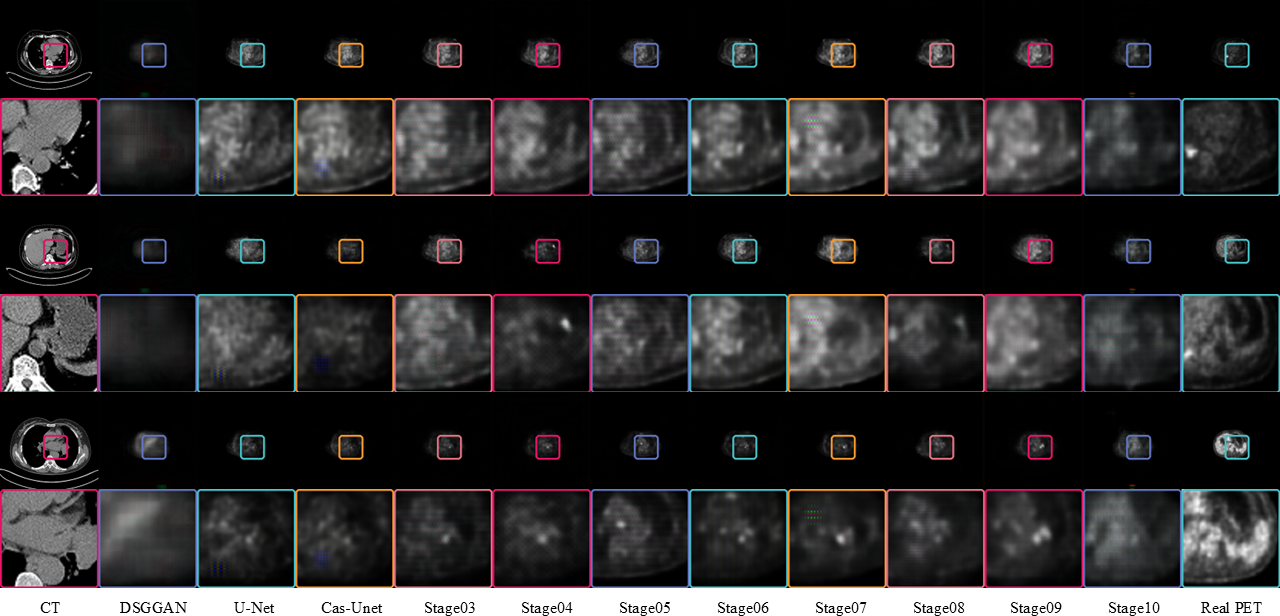
\includegraphics[width=1.0\linewidth]{u-net/lung/lung_compare_folder/lung_compare_13.png}
	% \caption[lung_compare]
	\caption[lung_compare]{The figure displayed here showcases PET images generated by various models, compared alongside real CT and PET images. The odd rows present the complete paired PET-CT images, while the even rows provide magnified views of specific regions within these pairs. Each model utilizes the CT image located at the extreme left as the input. The real PET images positioned at the extreme right serve as references for comparison. }
	\label{fig:lung_compare}
\end{figure*}
Visual comparisons (Figure \ref{fig:lung_compare}) indicated pixel-level metrics differed from perceived quality, highlighting artifacts in certain stages due to transpose convolutions. Quantitative metrics did not fully reflect visual quality, underscoring the need for expert evaluations or prior knowledge.

\section{Conclusion}
The proposed cascaded framework effectively enhanced performance and demonstrated stability. Future studies should integrate visual quality assessments and expert evaluations to increase practical utility in medical image translation tasks. The study's findings suggest that the multi-stage cascaded U-Net model can be a valuable tool for medical image synthesis, with potential applications in various medical imaging tasks. The results indicate that the model can effectively learn to generate high-quality images from CT scans, which could aid in improving diagnostic accuracy and treatment planning in clinical settings. Further research is needed to explore the model's performance on larger datasets and its applicability to other imaging modalities.

\section*{Acknowledage}
We would like to express our sincere gratitude to the National Cancer Institute Cancer Imaging Program for generously making their high-quality medical imaging dataset available and authorized for use on the Internet, providing indispensable resources for the smooth conduct of this research.

\bibliographystyle{unsrt}
\bibliography{unet_ref}

\end{document}
